\documentclass[american,9pt, landscape, a4paper, xcolor=table]{article}
%\usepackage{pgfpages}
%\pgfpagesuselayout{4 on 1}[a4paper,landscape,border shrink=4mm]

\usepackage{algcompatible}
%\usepackage{arrowsnew}
\usepackage{ulem,caption,longtable}

\newcommand{\high}[1]{\textcolor{red}{#1}}

\newcommand{\sk}[1]{}
\newcommand{\skn}[1]{#1}
\renewcommand{\sk}[1]{#1}
\renewcommand{\tilde}{\widetilde}
\newcommand{\lightning}{(contr.)}
\newcommand{\ca}{\operatorname{cap}}

\newcommand{\comment}[1]{%
\textcolor{black!40!white}{#1}}%
\newcommand{\alertline}{%
 \usebeamercolor[fg]{normal text}%
 \only{\usebeamercolor[fg]{alerted text}}}

%\usepackage{cmbrightmath, scaleupmath]{tpslifonts}
\newcommand\Loadedframemethod{default}
\usepackage[framemethod=tikz]{mdframed}

\usepackage[thicklines]{cancel}

\usepackage{tikz,pgf}
\usetikzlibrary{shapes.callouts,decorations.pathmorphing,arrows,snakes,shapes}
\usepackage{tikz-3dplot}
\usepgflibrary{shapes.callouts}

\usepackage[scale=0.9]{geometry}

\begin{document}


\pagestyle{empty}
~\hspace{-1cm}
\begin{tikzpicture}[scale=0.5,knoten/.style={circle, fill=yellow,scale=0.4},lab/.style={pos=0.5,fill=white,draw=black,scale=0.8,rectangle},edge/.style={thick,scale=0.1}]
\node (1) at (12.5,6.5) {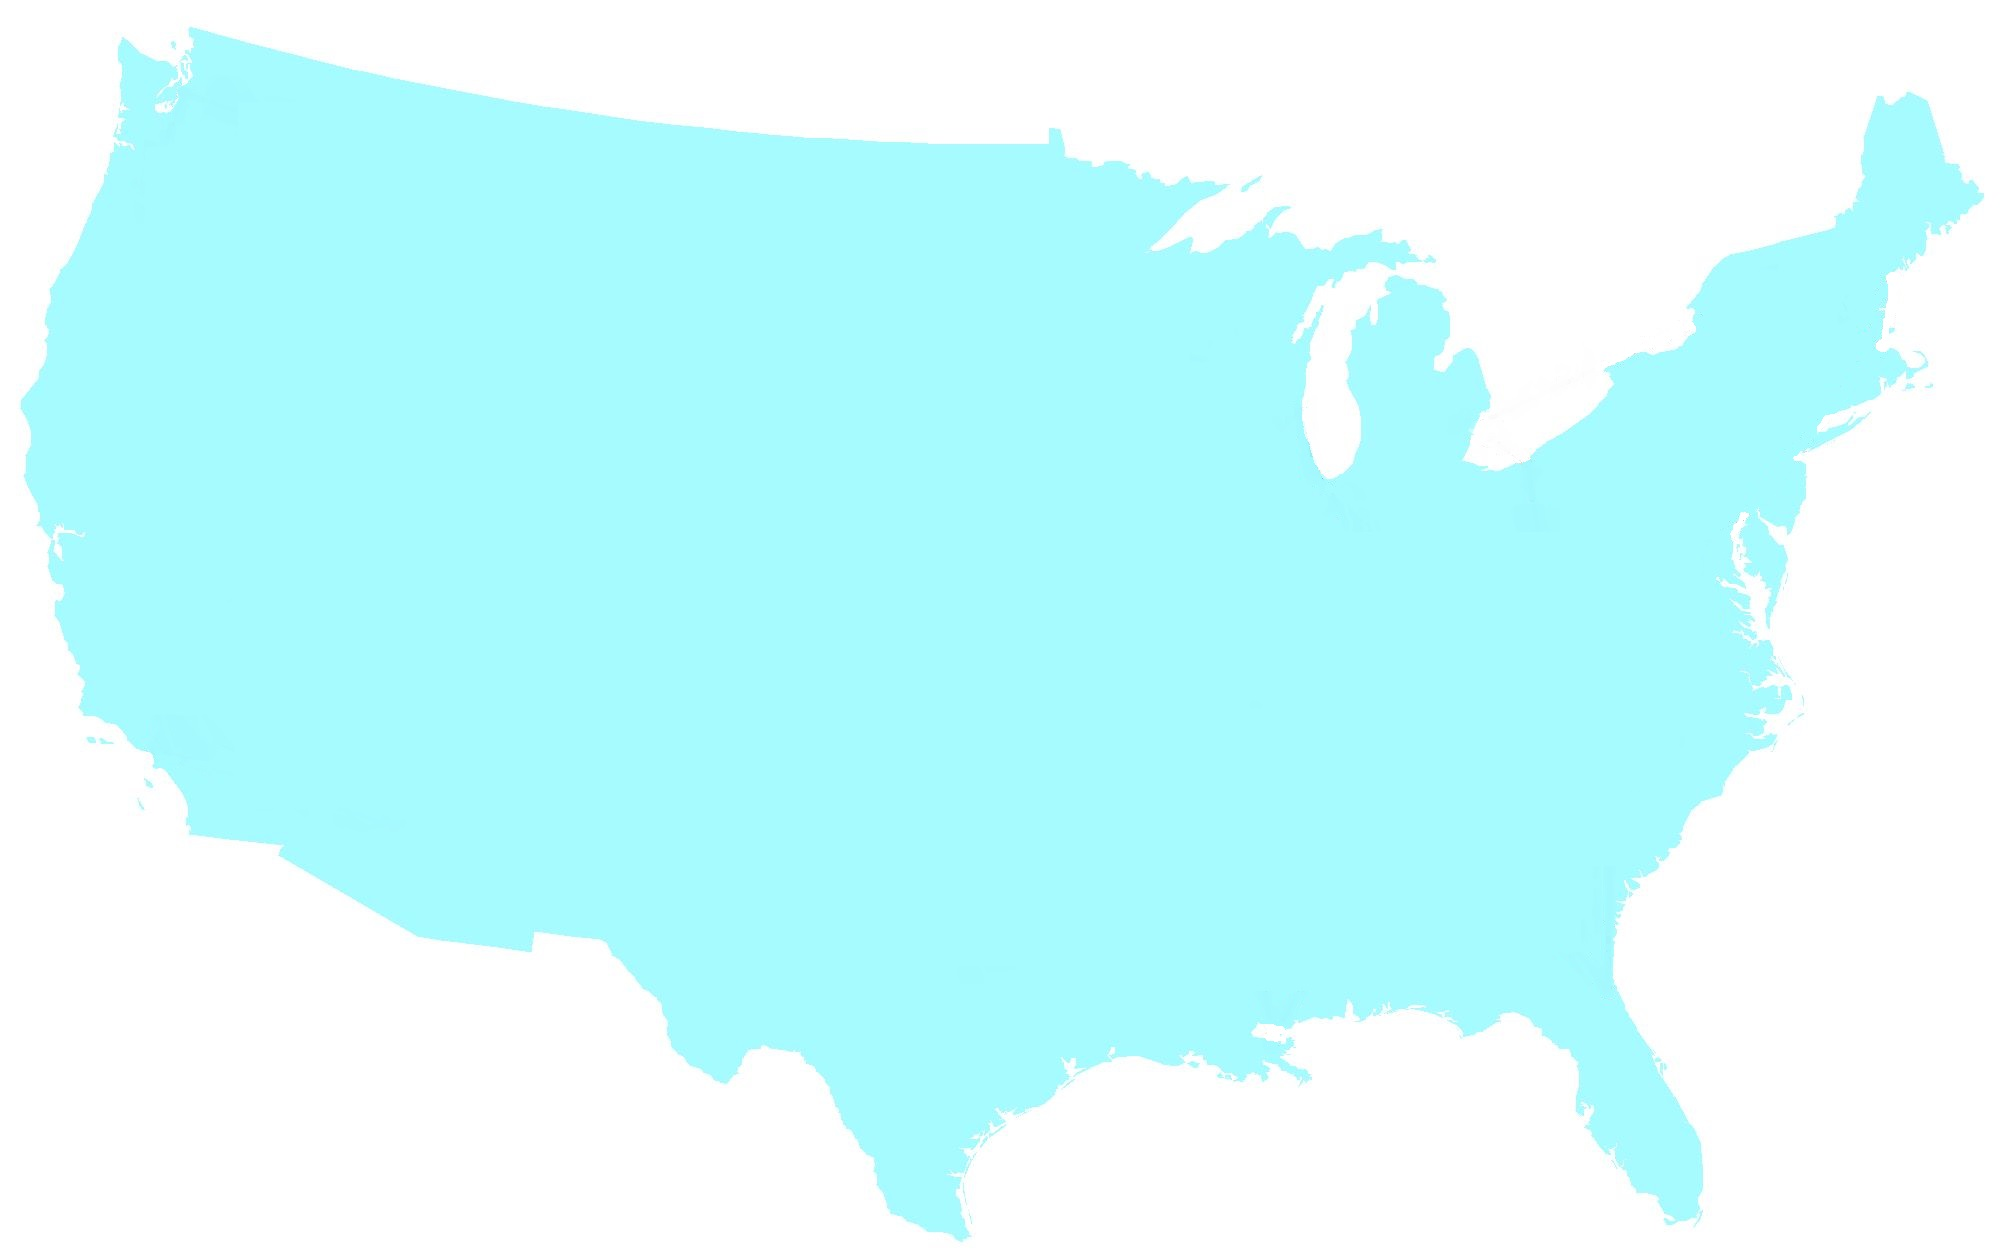
\includegraphics[scale=0.666]{country.jpg}};
%\node (1) at (12.5,6.5) {\includegraphics[scale=0.79]{dantzig_big.jpg}};

\node[knoten][label=above:1] (1) at (36.5,15.5) {1};
\node[knoten][label=above:2] (2) at (35.16,16.62) {2};
\node[knoten][label=above:3] (3) at (25.6,12.2) {3};
\node[knoten][label=above:4] (4) at (27.2,11.2) {4};
\node[knoten][label=above:5] (5) at (27.8,7) {5};
\node[knoten][label=above:6] (6) at (23.6,6.3) {6};
\node[knoten][label=above:7] (7) at (23,8.5) {7};
 \node[knoten][label=above:8] (8) at (21,11) {8};
 \node[knoten][label=above:9] (9) at (20.5,12.5) {9};
 \node[knoten][label=above:10] (10) at (15.5,15) {10};
 \node[knoten][label=above:11] (11) at (9,14) {11};
 \node[knoten][label=above:12] (12) at (8.5,17.5) {12};
 \node[knoten][label=above:13] (13) at (-1.5,18.5) {13};
 \node[knoten][label=above:14] (14) at (-10.5,21.5) {14};
 \node[knoten][label=above:15] (15) at (-11.5,19) {15};
 \node[knoten][label=above:16] (16) at (-6.5,15) {16};
 \node[knoten][label=above:17] (17) at (-3,10.5) {17};
\node[knoten][label=above:18] (18) at (-11,10) {18};
 \node[knoten][label=above:19] (19) at (-11.5,3) {19};
 \node[knoten][label=above:20] (20) at (-5,1) {20};
 \node[knoten][label=above:21] (21) at (2.5,3) {21};
 \node[knoten][label=above:22] (22) at (4,8.5) {22};
 \node[knoten][label=above:23] (23) at (4,10) {23};
 \node[knoten][label=above:24] (24) at (13,10) {24};
 \node[knoten][label=above:25] (25) at (15.5,10.5) {25};
 \node[knoten][label=above:26] (26) at (14.5,7) {26};
 \node[knoten][label=above:27] (27) at (13.5,7) {27};
\node[knoten][label=above:28] (28) at (11.5,2) {28};
 \node[knoten][label=above:29] (29) at (12,-1.5) {29};

 \node[knoten][label=above:30] (30) at (17,1) {30};
 \node[knoten][label=above:31] (31) at (19.5,2) {31};
 \node[knoten][label=above:32] (32) at (19.5,-2) {32};
 \node[knoten][label=above:33] (33) at (20,-5) {33};
 \node[knoten][label=above:34] (34) at (23,0) {34};
 \node[knoten][label=above:35] (35) at (25.5,0.5) {35};
 \node[knoten][label=above:36] (36) at (29.5,-3.5) {36};
 \node[knoten][label=above:37] (37) at (29.5,1.5) {37};
\node[knoten][label=above:38] (38) at (31.5,4) {38};
 \node[knoten][label=above:39] (39) at (32,6.5) {39};

 \node[knoten][label=above:40] (40) at (32.5,8.5) {40};
 \node[knoten][label=above:41] (41) at (37,14.5) {41};
 \node[knoten][label=above:42] (42) at (37.5,16.5) {42};

\draw[edge] (2) to node[lab]{1} (1);
\draw[edge] (4) to node[lab]{1} (3);
\draw[edge] (5) to node[lab]{0.5} (4);
\draw[edge] (6) to node[lab]{0.5} (4);
\draw[edge] (6) to node[lab]{0.5} (5);
\draw[edge] (7) to node[lab]{1} (6);
\draw[edge] (8) to node[lab]{1} (7);
\draw[edge] (9) to node[lab]{1} (3);
\draw[edge] (9) to node[lab]{1} (8);
\draw[edge] (12) to node[lab]{1} (10);
\draw[edge] (12) to node[lab]{1} (11);
\draw[edge] (14) to node[lab]{1} (13);
\draw[edge] (15) to node[lab]{1} (14);
\draw[edge] (16) to node[lab]{0.5} (15);
\draw[edge] (17) to node[lab]{1} (13);
\draw[edge] (17) to node[lab]{1} (16);
\draw[edge] (18) to node[lab]{0.5} (15);
\draw[edge] (18) to node[lab]{0.5} (16);
\draw[edge] (19) to node[lab]{1} (18);
\draw[edge] (20) to node[lab]{1} (19);
\draw[edge] (21) to node[lab]{1} (20);
\draw[edge] (22) to node[lab]{1} (21);
\draw[edge] (23) to node[lab]{1} (11);
\draw[edge] (23) to node[lab]{1} (22);
\draw[edge] (25) to node[lab]{1} (10);
\draw[edge] (25) to node[lab]{1} (24);
\draw[edge] (27) to node[lab]{1} (24);
\draw[edge] (27) to node[lab]{1} (26);
\draw[edge] (28) to node[lab]{1} (26);
\draw[edge] (29) to node[lab]{1} (28);
\draw[edge] (30) to node[lab]{1} (29);
\draw[edge] (31) to node[lab]{1} (30);
\draw[edge] (32) to node[lab]{1} (31);
\draw[edge] (33) to node[lab]{1} (32);
\draw[edge] (34) to node[lab]{1} (33);
\draw[edge] (35) to node[lab]{1} (34);
\draw[edge] (36) to node[lab]{1} (35);
\draw[edge] (37) to node[lab]{1} (36);
\draw[edge] (38) to node[lab]{1} (37);
\draw[edge] (39) to node[lab]{1} (38);
\draw[edge] (40) to node[lab]{1} (5);
\draw[edge] (40) to node[lab]{1} (39);
\draw[edge] (41) to node[lab]{1} (1);
\draw[edge] (42) to node[lab]{1} (2);
\draw[edge] (42) to node[lab]{1} (41);

\end{tikzpicture}




\end{document}
